
% STATEMENTS
\begin{frame}
	\Section{Mathematical Basics}
	In this first section we will provide mathematical notations and concepts which are fundamental and crucial for the further presentation.\\
	\vspace{0.2cm}
	\Subsection{Statements}
		\vspace{0.2cm}
	By a \textbf{statement} we mean a linguistic or mental construction that is either true or false.
	\vspace{0.2cm}
	\begin{ex}~\\\vspace{0.1cm}
		\ite
		\item ``4 is an even number.'' is a true statement.
		\item ``Bananas have conic shape.'' is a false statement.
		\item ``In the night, it is colder than outside.'' is not a statement.
		\item ``There are infinitely many stars.'' is a statement, which can be true or false.
		\eti
	\end{ex}
	\vspace{0.2cm}
	\textbf{Relations and Operations}
	\color{defgruen}
	\begin{center} \vspace{-0.1cm}
		\begin{tabular}[t]{ll}
			$\neg A$: & $A$ is false (\textbf{negation})\\\vspace{0.2cm}
			$A\RA B$: & from $A$ follows $B$; if $A$ is true, then also $B$ is true (\textbf{implication})\\\vspace{0.2cm}
			& we say: $A$ is \textbf{sufficient} for $B$, $B$ is \textbf{necessary} for $A$\\\vspace{0.2cm}
			$A\LRA B$: & $A$ is true, if and only if  $B$ is true. (\textbf{equivalence})
		\end{tabular}
	\end{center}
\color{fontcolor}
	Note that the following two statements are equivalent
	\begin{align*}
	\color{satzrot}A&\color{satzrot}\RA B\\
	\color{satzrot}\neg B&\color{satzrot} \RA \neg A 
	\end{align*}
	{
\blank
For example $A$: ``it rains'', $B$: ``the street is we'', then $\neg A$: ... and $\neg B:$ ...	
}
\end{frame}

\mode<article>{
\begin{center} \vspace{-0.1cm}
	\begin{tabular}[t]{ll}
		$A\wedge B$: & $A$ and $B$ are true (\textbf{and})\\
					$A\vee B$: & $A$ or $B$ is true (\textbf{or})\\
					$A\:\dot\vee\: B$: & either $A$ or $B$ is true (\textbf{excl. or})\\

	\end{tabular}
\end{center}
}

\begin{frame}
\Subsection{Sets}
 \begin{defi}[Set]\label{def:set}
 	According to \textsc{Cantor}\index{Cantor@\textsc{Cantor}} a \textbf{set} is a well-defined collection of distinct objects, considered as an object in its own right. The objects that make up a set (also known as the set's \textbf{elements}) can be anything: numbers, people, letters of the alphabet, other sets, and so on. 	 
 \end{defi}
\vspace{0.1cm}
 \textbf{Notation:} curly brackets $\{ \}$
 \vspace{0.1cm}
 \begin{ex} \label{ex:sets}~\\
 	\blank
 	\begin{itemize}
 		\blank
 		\item[\blank$\bullet$] $M := \{ 1,2,3 \}$
 		\item[\blank$\bullet$] $N := \{ \underbrace{x}_{\text{\scriptsize element}} \,|\, \underbrace{\text{$x$ is multiple of } ~7}_{\text{\scriptsize element property}} \}= \{ x \,\colon\, \text{$x$ is multiple of }~ 7 \} = \{7,14,21,\ldots\}$ \vspace{0.2cm}
 	\end{itemize}
  $\rightarrow$ Note: We use ``$:=$'' for definitions\\
 \end{ex}
\vspace{0.6cm}
\begin{defi}[Cardinality]\label{def:cardinality}
If a set $M$ is \textbf{finite} (i.e., it only contains finitely many elements), then we denote by $|M|$ the number of elements contained in $M$ and call it \textbf{cardinality of $M$}.
\end{defi}
\end{frame}

\begin{frame}
\textbf{\large Set relations and further definitions}\\
\vspace{0.2cm}
\begin{table}[h] \color{defgruen}
	\begin{tabular}[t]{ll}
		$a \in M$ (or $M \ni a$): & $a$ is element of $M$; $M$ contains $a$\\\vspace{0.2cm}
		$a \not\in M$ (or $M \not\ni a$): & $a$ is not element of $M$; $M$ does not contain $a$
	\end{tabular}
\end{table}	 
{\blank
$M = \{1,2,3\}$, $1 \in M$, $\{1\} \notin M$
	\vspace*{0.4cm}
}
\begin{table}[h] \color{defgruen}
	\begin{tabular}[t]{ll}
		$M=N$: & $M$ contains the same elements as $N$\\\vspace{0.2cm}
		$M\not=N$: & $M$ does not contain the same elements as $N$
	\end{tabular}
\end{table}

{\blank
	$N := \{1,2\}$,  $M=M$, $M \neq N$
	\vspace*{0.4cm}
}

\begin{table}[h] \color{defgruen}
	\begin{tabular}[t]{ll}
		$M \subset N$ (or $M\subseteq N$): & $M$ is subset of $N$, i.e., each element of $M$ is also \\\vspace{0.2cm}
		& an element of $N$; equality of sets is permitted.\\\vspace{0.2cm}
		$N \supset M$ (or $N\supseteq M$): & $N$ is superset of $M$; analogously\\\vspace{0.2cm}
		$M \subsetneqq N$: & $M$ is strict subset of $N$; $M\not=N$\\\vspace{0.2cm}
		$\emptyset = \{\}$: & empty set
	\end{tabular}
\end{table}
{\blank
	$N \subset M$ and even $N \subsetneqq M$; what about the relation between $N_2 :=\{\{1\}, 2\}\}$ and  $M$ or $\emptyset$ and  $M$?
\vspace*{0.4cm}
}
~\\
\textbf{Remark:} Very useful in practice to show that two sets are equal: \\
$$M=N \iff M\subset N \textbf{~~and~~} N \subset M $$
\end{frame}

\begin{frame}
	\begin{table}[h] \color{defgruen}
		\begin{tabular}[t]{ll}
			$M \times N$: & \textbf{cartesian product} defined by 
			$M \times N :=\{(m,n)\colon m\in M,n\in N  \}$\vspace{0.2cm}\\\vspace{0.4cm}
			& $M^n := M \times \ldots \times M$ ($n$ times)
		\end{tabular}
	\end{table}
{
	\blank
Let us consider $$M:=\{ x : \text{$x$ is multiple of } ~2 \} = \{2, 4, 6, \ldots\}$$ and 
$$N:=\{ x : \text{$x$ is multiple of } ~4 \} = \{4, 8, 12, \ldots\},$$ then we have\\ 
$$M \times N = \{(a,b): a\in M, ~b\in N\} = \{ (2,4), (2,8),\ldots, (4,4), (4,8), \ldots \}$$ \\~\\
\textit{(depict regular Cartesian grid)}
}
\end{frame}

\begin{frame}
\begin{table}[h] \color{defgruen}
	\begin{tabular}[t]{ll}
	$\mathcal{P} (M)$  & \textbf{power set of $M$} defined by\\
	&$\mathcal{P} (M) := 2^M :=\{ N: N\subset M\} $ (set of all subsets of $M$)\\
	&\vspace{0.2cm}We find $|\mathcal{P} (M)| = 2^{|M|}$
\end{tabular}
\end{table}
{
	\blank~\\

 Let us consider $M=\{ 1,2\}$, then $|M|=2$ and the power set of $M$ is given by
	\[\mathcal{P}(M)=2^M=\bigl\{\emptyset ,\{ 1\},\{ 2\},\{ 1,2\}\bigr\}.\]
	We also find
	$$|\mathcal{P}(M)|=4 = 2^{|M|}=2^2 . $$
	~\\
	Remark: \textbf{Binomial theorem}
	$$ \sum_{k=0}^n 	\binom{n}{k} =2^n,  $$
	where $$\binom{n}{k} := \frac{n!}{k!(n-k)!}$$ is the so-called binomial coefficient, which give us the number of subsets with $k$ elements that we can draw from a set with $n$ elements.

}
\end{frame}



\begin{frame}
	\textbf{\large Summary: Set relations and further definitions}\\
	\vspace{0.2cm}
	\begin{table}[h] \color{defgruen}
		\begin{tabular}[t]{ll}
			$a \in M$ (or $M \ni a$): & $a$ is element of $M$; $M$ contains $a$\\\vspace{0.2cm}
			$a \not\in M$ (or $M \not\ni a$): & $a$ is not element of $M$; $M$ does not contain $a$\\[3pt]
			$M=N$: & $M$ contains the same elements as $N$\\\vspace{0.2cm}
			$M\not=N$: & $M$ does not contain the same elements as $N$\\\vspace{0.2cm}
			$M \subset N$ (or $M\subseteq N$): & $M$ is subset of $N$, i.e., each element of $M$ is also \\\vspace{0.2cm}
			& an element of $N$; equality of sets is permitted.\\\vspace{0.2cm}
			$N \supset M$ (or $N\supseteq M$): & $N$ is superset of $M$; analogously\\\vspace{0.2cm}
			$M \subsetneqq N$: & $M$ is strict subset of $N$; $M\not=N$\\\vspace{0.2cm}
			$\emptyset = \{\}$: & empty set\\\vspace{0.2cm}
			$M \times N$: & \textbf{cartesian product} defined by 
			$M \times N :=\{(m,n)\colon m\in M,n\in N  \}$\\\vspace{0.4cm}
			& $M^n := M \times \ldots \times M$ ($n$ times)\\\vspace{0.2cm}
			$\mathcal{P} (M)$  & \textbf{power set of $M$} defined by\\
			&$\mathcal{P} (M) := 2^M :=\{ N: N\subset M\} $ (set of all subsets of $M$)\\
			&\vspace{0.2cm}We find $|\mathcal{P} (M)| = 2^{|M|}$
		\end{tabular}
	\end{table}
\end{frame}






\begin{frame} 
\textbf{\large Set operations} ~\\ 
\vspace{0.2cm}
$$\begin{array}{llll} 
M \cup N &:=& \lbrace a: a\in M \text{ or } a \in N\rbrace&\text{(\textbf{\color{defgruen}union})}\\[3pt]
M \cap N &:=& \lbrace a: a\in M \text{ and } a \in N\rbrace&\text{(\textbf{\color{defgruen}intersection})}\\[3pt]
M \setminus N &:=& \lbrace a : a\in M \text{ and } a \not\in N\rbrace&\text{(\textbf{\color{defgruen}difference})}\\[6pt]
\text{If}~N\subset M&&&\\[6pt]
 N^c  &:=&  \overline{N}:= M \setminus N&\text{(\textbf{\color{defgruen}complement of N with respect to M})}\\[3pt]
%  M \dot\cup N &=& M \cup N  \text{~~if~~} M\cap N = \emptyset  &  \text{(disjoint union)}
\end{array}$$ 
~\\\vspace{0.3cm}
$M, N$ are called \textbf{\color{defgruen}disjoint}\index{disjoint},  if $M \cap N = \emptyset$.
%
\vspace{0.5cm}
\begin{ex} \label{ex:set_operations}
	~\\
	\blank
	Let $M = \{1,2,3, 4\}$ and $N = \{1,3\}$, then\vspace{0.2cm}
	\begin{itemize}
		\blank
		\item[] $M \cup N = \{1,2,3, 4\}$, we always have $M \subset M\cup N$ and  $N \subset M\cup N$ \vspace{0.2cm}
		\item[] $M \cap N = \{1, 3\}$\vspace{0.2cm}
		\item[] $\overline{N} =M \setminus N = \{2, 4\}$
	\end{itemize}
\end{ex}
\vspace{0.2cm}

\end{frame}

% DE MORGAN
\begin{frame}
For combinations of those set operations we have the following result: \vspace{-0.2cm}
 \begin{lemma}[\textbf{\textit{De Morgan's laws}}]\label{lem:demorgan}
 	Let $\Omega$ be a set and $M,N \subset \Omega$. Then we find
 	\begin{itemize}
 		\item[i)] $ (M\cup N)^c  = M^c \cap N^c $,
 		\item[ii)] $ (M\cap N )^c =  M^c \cup  N^c $.
 	\end{itemize}
 Here the complements are taken with respect to $\Omega$.
 \end{lemma}\vspace{-0.5cm}
 \begin{proof}
 	\textit{Exercise.}
 \end{proof}
{
	\blank
	~\\
	Illustration:\\
	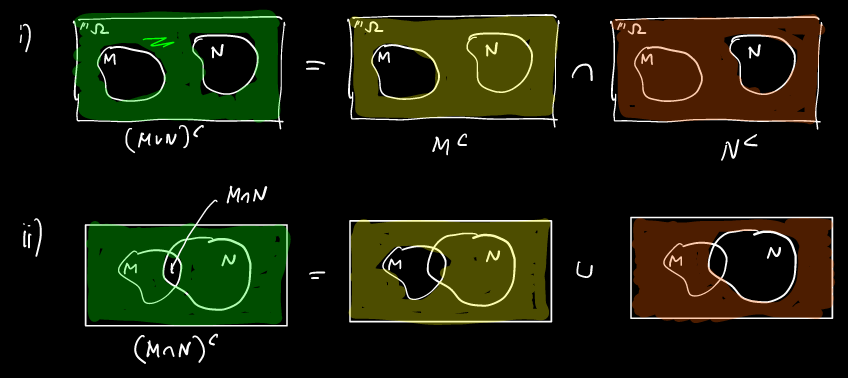
\includegraphics[width=0.8\textwidth]{\PathToMedia/venn-diagram.png}
}
\end{frame}
 
\begin{frame}
%functionS
\Subsection{Functions}
\begin{defi}[\textbf{\textit{function}}]\label{def:function}
	Let $M, N$ be two sets. A \textbf{function} or \textbf{mapping} $f$ from $M$ to $N$ (notation: $f\colon M\to N$) is determined by
	\begin{itemize}
		\item[] its \textbf{domain} $M$, 
		\item[] its \textbf{codomain} $N$,
		\item[] and a \textbf{rule},
	\end{itemize} 
that uniquely assigns to each element $a\in M$ an $b:=f(a)\in N$ (notation: $a \mapsto f(a)$).	 
\end{defi}
Two functions $f_1: M_1\to N_1$ and $f_2: M_2\to N_2$ are called \textbf{equal} (abbr.~$f_1\equiv f_2$) (identical),
if $M_1=M_2$, $N_1=N_2$ and $f_1(a)=f_2(a)$ for all $a\in M_1$ (i.e., equal, domain, codomain and rule).
%
	
\vspace{0.4cm}
\begin{ex}\label{ex:image_preimage_graph}
	~\\
	\blank
	Let $M := N :=\{1,2,3,4,5\ldots\}$ and consider $f\colon M \to N,~ a \mapsto 2a$. How could we ``visualize'' this function?\\ \vspace{0.2cm}
	i) a \textbf{table} with two columns (one for domain and codomain each)
	\begin{itemize}
		\blank
		\item[] follow where points go from $A=\{1,2\}\subset M$ 
		\item[] find points which would produce $B=\{4,6\} \subset N$
	\end{itemize}\vspace{0.2cm}
	ii) draw the \textbf{graph} into a coordinate system
\end{ex}
\end{frame}

\begin{frame}
	We introduce function related sets: \vspace{-0.3cm}
	\begin{defi}[{\textit{Image, preimage, graph}}]\label{def:image_preimage_graph}
		Let $A \subset M$ and $B \subset N$, then
		\begin{itemize} \color{defgruen}
			\item[i)] the set $f(A) = \{f(a) : a\in A\} \subset N$ is called \textbf{image set} of $A$ (under $f$),
			\item[ii)] the set $f^{-1}(B)=\lbrace a\in M: f(a)\in B\rbrace \subset M$ is called \textbf{preimage} of $B$ (under $f$),
			\item[iii)] the set $\text{graph}(f) := \{(a,f(a))\colon a \in M\} \subset M\times N$ is called the \textbf{graph} of $f$.
		\end{itemize} 
	\end{defi}
	$\rightarrow$ \textbf{Attention:} Here, $f^{-1}$ is not the inverse function (see below).\\ \vspace{0.2cm}
	{\blank
	i) abstract picture with  with image, preimage and graph\\
	ii) With the definitions from above we have
	\begin{itemize}
		\blank
		\item[] for $A=\{1,2\}$ we find $f(A) = \{2,4\}$
		\item[] for $B=\{4,6\}\}$ we find $f^{-1}(B) = \{2,3\}$
		\item[] $\text{graph}(f) = \{(1,2), (2,4), (3,6), \ldots\}$
	\end{itemize}
}	
\end{frame}


 
\begin{frame}
Important properties of functions: \vspace{-0.3cm}
\begin{defi}[\textbf{\textit{Injective, surjective, bijective}}] \label{def:injective_surjective_bijective}
	A function 	$f: M\to N$ is called
	\ite
	\item[i)] \textbf{injective} (one-to-one), if $f(a)\not=f(\tilde a)$ for all $a,\tilde a\in M$ with $a\not=\tilde a$;
	\item[ii)] \textbf{surjective} (onto), if for all $b\in N$ there exists an $a\in M$ with $f(a)=b$ (or equivalently $f(M)=N$);
	\item[iii)] \textbf{bijective}, if $f$ is injective as well as surjective  relation.
	\eti 
\end{defi}
%
\vspace{0.3cm}
We can invert bijective functions:\vspace{-0.3cm}
\begin{defi}[\textbf{\textit{Inverse function}}] \label{def:composition}
	Let $f\colon M\to N$ be a bijective (invertible) function. Then there exists a (unique) function $f^{-1}\colon N \to M$, the so-called \textbf{inverse of $f$}, such that
	$$f(a) = b \iff f^{-1}(b) = a.$$ 
\end{defi}
%
\vspace{0.3cm}
\begin{ex}
	\blank
 Consider again example from above and the visualization with the help of the table.
\end{ex}
\end{frame}

\begin{frame}
\vspace{0.3cm}
We can concatenated two or more functions:\vspace{-0.3cm}
\begin{defi}[\textbf{\textit{Composition}}] \label{def:composition}
	Let $f\colon M\to N$ and $g\colon N\to P$ be functions, then we call the function
	$$g\circ f\colon M\to P,~ a \mapsto g(f(a))$$
	\textbf{composition} of $f$ and $g$. 
\end{defi}
%
{	\blank
	~\\
	i) abstract picture for composition of the functions\\
	ii) Concrete example:
	\begin{align*}
	&M=\{1,2,3,4,\dots\},~N:=\{x:~x~\text{is even}\},~P:=\{x:~x~\text{is odd}\},\\
	&f:M\rightarrow N, a\mapsto 2a,~g:N\rightarrow P, b\mapsto b-1
	\end{align*}
	$$
	(g\circ f)(6)=g(\underbrace{f(6)}_{=12})=g(12)=12-1=11
	$$
}
\noindent A function with ``no effect'':\vspace{-0.3cm}
\begin{defi}[\textbf{\textit{Identity function}}] \label{def:identity}
	Let $M$ be a set. Then the function 
	$$id := id_M \colon M \to M, ~a\mapsto a $$
	is called the \textbf{identity function on $M$}.
\end{defi}

 \end{frame}





% QUANTORS and AIM of MATH
\only<article>{
\begin{frame}
If $M$ is a set and $P$ a property, which an element $a\in M$ can have. Then, we use the abbreviations for certain statements: 
\ite
\item {\color{defgruen}$\forall {a\in M}\,:\, a$ has property $P$}\\
means: each $a\in M$ has property $P$ \qquad
(``$\forall$'' is called \textbf{all quantor})
\item {\color{defgruen}$\exists {a\in M}\,:\, a$ has property $P$}\\
means: there is at least one $a\in M$ with property $P$\qquad
(``$\exists$'' is called \textbf{existence quantor})
\item {\color{defgruen}$\exists_1{a\in M}\,:\, a$ has property $P$}\\
means: there is  \textbf{exactly one} $a\in M$ with property $P$
\eti
%
\vspace{0.3cm}
Note the interesting equivalences
\begin{align*}
\color{satzrot}\neg(\forall {a\in M}\,:\, a \text{ has property }P)& \color{satzrot}\Longleftrightarrow \exists {a\in M}\,:\, a \text{ does not have property }P\\
\color{satzrot}\neg(\exists {a\in M}\,:\, a \text{ has property }P)& \color{satzrot}\Longleftrightarrow \forall {a\in M}\,:\, a \text{ does not have property }P
\end{align*}
\begin{ex}\label{ex:quantors}
	\blank
	content...
\end{ex}
%
\textit{Aim of mathematics: make nontrivial statements about certain structural objects.
	However, its whole theoretical construction cannot be founded on nothing. As a foundation, we formulate a minimum number of plausible axioms, which are not and cannot be proved.}
\textit{In particular, we need axioms for the definition of \textbf{numbers.} The \textsc{Peano} axioms give the natural numbers $\N$, from which negative and rational numbers can be constructed. A further axiom gives the real numbers $\R$. }
 \end{frame}
}



 

 
\begin{frame}
\Subsection{Numbers} \label{numbers}
%\only<presentation>{	\tableofcontents[currentsubsection]}
The notion of \textbf{number} has been extended over the centuries, here we do not go in detail through the axiomatic construction but just point out some properties that are useful in the remaining.\\
\vspace{0.5cm}
Here is an overview:\\
\begin{table}
	\centering
	\begin{tabular}{c|c|c|l}
		$\N$ & \textbf{Natural} 	& $\{1,2,3,4, 5, \ldots\}$ & counting objects\\
		&&&\textbf{order relation}: $m\le n$\\
		&&&$m+n$, $m\cdot n$\\
		&&&proof concept of \textbf{induction} \\[0.3cm]
		%
		$\Z$ & \textbf{Integer} 	& $\{ \ldots,-3,-2,-1,0,1,2,3, \ldots\}$ & adding zero and negative numbers (borrowing money,...)\\ 
		&&&$(\Z, +)$ \textbf{ordered, commutative group}\\[0.3cm]
		%
		$\Q$ & \textbf{Rational} & $\left\lbrace \frac{p}{q}: ~p,q\in \Z, q \neq 0 \right\rbrace $& adding fractions of objects (one half of a cake)\\
		&&&$(\Q, +, \cdot)$ \textbf{ordered field}\\[0.3cm]
		%
		$\R$ & \textbf{Real} 	& $ \Q \cup \{\text{limits of sequences in } \Q\}$ & adding square roots ($\sqrt{2}$,$\sqrt{5}$,...), $\pi$,...\\
		&&&$(\R, +, \cdot)$ \textbf{ordered and complete field} \\[0.3cm]
		%
		$\C$ & \textbf{Complex}  & $\{a+ib:~a,b\in \R\}$, $i:= \sqrt{-1}$  & adding e.g. square root of negative numbers\\
		&&&$\R \times \R$~ \text{with a special multiplication}\\
		&&&$(\C,+, \cdot)$ \textbf{complete field} (not ordered)
	\end{tabular}
	\label{tab:numbers}
\end{table}
We have
$$\N ~~\subsetneqq~~ \Z~~  \subsetneqq~~   \Q ~~ \subsetneqq ~~  \R~~  \subsetneqq~~  \C $$ 
\end{frame}

\only<article>{
% NATURAL NUMBERS and % INTEGERS
\begin{frame}
\Subsubsection{Natural Numbers $\N$}
\vspace{0.5cm}
$\color{defgruen}\N:=\{1,2,3,\ldots\}$
\vspace{0.5cm}
\begin{itemize}
	\item most intuitive concept; counting objects \vspace{0.2cm}
	\item in mathematics rigorously defined through \textbf{the Dedekind-Peano Axioms} \vspace{0.2cm}
	\item (binary) operations on natural numbers: \vspace{0.2cm}
	\begin{itemize}  \normalsize
		\item summation: $m+n$ (commutative) \vspace{0.2cm}
		\item multiplication $m \cdot n$ (commutative) \vspace{0.2cm}
	\end{itemize}
	\item The natural numbers have an \textbf{order relation}: $m\le n$	 \vspace{0.2cm}
	\item Each natural number has a successor and thereby gives the proof concept of \textbf{induction}
\end{itemize}
\vspace{0.5cm}
\end{frame}

\begin{frame}
\Subsubsection{Integers $\Z$}
\vspace{0.5cm}
$\color{defgruen}\Z:=\{\ldots ,-3,-2,-1,0,1,2,3,\ldots\}$
\vspace{0.5cm}
\begin{itemize}
	\item extension: zero and negative numbers 
	\item in real life, negative numbers exist only in relations: borrowed money, i.e., wealth difference of the borrower
	\item (binary) operations on integers:
	\begin{itemize} \normalsize
		\item summation: $z+w$ (commutative)
		\item multiplication $z \cdot w$ (commutative)
	\end{itemize}
	\item integers have an \textbf{order relation}: $m\le n$
	\item $(\Z, +)$ gives a so-called (commutative) \textbf{group} 
\end{itemize}
\end{frame}


\begin{frame}
\Subsubsection{Rational Numbers $\Q$}
\vspace{0.5cm}
$\color{defgruen}\Q:=\left\lbrace \frac{p}{q}: p,q\in\Z, q\neq 0\right\rbrace $
\vspace{0.5cm}
\begin{itemize}
	\item extension: fractions $\frac{1}{2},\frac{5}{7},... $
	\item in real life, negative numbers exist only in relations: tax payment in relation to overall income
	\item (binary) operations on integers:
	\begin{itemize} \normalsize
		\item summation: $\frac{p}{q} + \frac{z}{w} = \frac{wp + qz}{qw}$ (commutative)
		\item multiplication $\frac{p}{q} \cdot \frac{z}{w} = \frac{pz}{qw}$ (commutative)
	\end{itemize}
	\item Rational numbers have an \textbf{order relation}: $m\le n$
	\item $(\Q, +)$ forms a (commutative) \textbf{group}
	\item $(\Q\backslash \{0\}, \cdot)$ forms a (commutative) \textbf{group} 
	
	\item $(\Q,+, \cdot)$ is a so-called (ordered) \textbf{field}, since $+$ and $\cdot$ are connected by the \textbf{distributive law}
	\[\color{satzrot}
	\frac{p_1}{q_1}\cdot \left(\frac{p_2}{q_2}+\frac{p_3}{q_3}\right)=
	\frac{p_1}{q_1}\cdot \frac{p_2}{q_2}+\frac{p_1}{q_1}\cdot \frac{p_3}{q_3}.
	\]	
\end{itemize}
%\vspace{0.8cm}
%\small
%--------------------------------------------------------------------------------------------------------------------------------\\
%\vspace{-0.3cm}
%\begin{defi}[Field]\label{def:field} 
%	Let $\F$ be a set and $\star$ as well as $\bullet$  binary operations on $\F$, then $(\F, \star, \bullet)$ is called a \textbf{field}, if
%	\begin{itemize}
%		\item[i)] $(\F, \star)$ is a commutative group,
%		\item[ii)] $(\F\setminus \{0\}, \bullet)$ is a commutative group,
%		\item[iii)] distributive law: $g_1 \bullet ( g_2 \star g_3) =g_1 \bullet  g_2 \star g_1 \bullet  g_3$.
%	\end{itemize}
%\end{defi}
\end{frame}

\begin{frame}
\Subsubsection{Real Numbers $\R$}
\vspace{0.5cm}
$\color{defgruen} \R = \text{``}\Q \cup \{\text{limits of sequences in } \Q\} \text{''}$
\vspace{0.5cm}
\begin{itemize}
\item extension: e.g., $\sqrt{2}, \sqrt{3},\ldots, \pi, e ~~\in\R\setminus\Q$
\item in real life: constant edge ratio of DIN-A format is $\sqrt{2}$
\end{itemize}
\vspace{0.5cm}
$\R$ inherits the following properties from $\Q$: \\\vspace{0.2cm}
\begin{itemize}
\item (binary) operations on real numbers:
\begin{itemize} \normalsize
	\item summation: $x+y$ (commutative)
	\item multiplication $x \cdot y$ (commutative)
\end{itemize}
\item Real numbers have an \textbf{order relation}: $m\le n$ \vspace{0.2cm}
\item $(\R, +)$ forms a (commutative) \textbf{group} \vspace{0.2cm}
\item $(\R \backslash \{0\}, \cdot)$ forms a (commutative) \textbf{group} \vspace{0.2cm}
\item $(\R,+, \cdot)$ forms a (ordered and \textit{complete}) \textbf{field} \vspace{0.2cm}
\end{itemize}
\end{frame}
}



%%%%%%%%%%%%%%%%%%%%%%%%%
% NUMBERS in article
\only<article>{
	% NATURAL NUMBERS and % INTEGERS
	\begin{frame}
	\Subsubsection{Natural Numbers $\N$}
	\vspace{0.5cm}
	$\color{defgruen}\N:=\{1,2,3,\ldots\}$
	\vspace{0.5cm}
	\begin{itemize}
		\item most intuitive concept; counting objects \vspace{0.2cm}
		\item in mathematics rigorously defined through \textbf{the Dedekind-Peano Axioms} \vspace{0.2cm}
		\item (binary) operations on natural numbers: \vspace{0.2cm}
		\begin{itemize}  \normalsize
			\item summation: $m+n$ (commutative) \vspace{0.2cm}
			\item multiplication $m \cdot n$ (commutative) \vspace{0.2cm}
		\end{itemize}
		\item The natural numbers have an \textbf{order relation}: $m\le n$	 \vspace{0.2cm}
		\item Each natural number has a successor and thereby gives the proof concept of \textbf{induction}
	\end{itemize}
	\vspace{0.5cm}
\end{frame}

\begin{frame}
\Subsubsection{Integers $\Z$}
\vspace{0.5cm}
$\color{defgruen}\Z:=\{\ldots ,-3,-2,-1,0,1,2,3,\ldots\}$
\vspace{0.5cm}
\begin{itemize}
\item extension: zero and negative numbers 
\item in real life, negative numbers exist only in relations: borrowed money, i.e., wealth difference of the borrower
\item (binary) operations on integers:
\begin{itemize} \normalsize
	\item summation: $z+w$ (commutative)
	\item multiplication $z \cdot w$ (commutative)
\end{itemize}
\item integers have an \textbf{order relation}: $m\le n$
\item $(\Z, +)$ gives a so-called (commutative) \textbf{group} 
\end{itemize}

\vspace{1.5cm}
\small
-------------------------------------------------------------------------------------------------------------------------------------\\
\vspace{-0.3cm}
\begin{defi}[Group]\label{def:group} 
Let $G$ be any set and $\star$ a binary operation on $G$, so that $g_1 \star g_2 \in G$, then $(G, \star)$ is called a \textbf{group}, if
\begin{itemize}
	\item[i)] associativity: $\forall g_1, g_2, g_3 \in G:~~ g_1 \star (g_2 \star g_3) = (g_1 \star g_2) \star g_3$,
	\item[ii)] neutral element: $\exists e \in G ~\forall g\in G:~~ g \star e = g$,
	\item[iii)] inverse element: $\forall g\in G ~\exists g^{-1}\in G:~~ g \star g^{-1} = e$,
	\item[iv)] $G$ is additionally called \textbf{commutative}, if $~\forall g_1, g_2\in G:~g_1 \star g_2  = g_2 \star g_1  $.
\end{itemize}
\end{defi}
This is not just an abstract notion: Modern cryptography is heavily based on group theory!
\end{frame}
	
	\begin{frame}
	\Subsubsection{Rational Numbers $\Q$}
	\vspace{0.5cm}
	$\color{defgruen}\Q:=\left\lbrace \frac{p}{q}: p,q\in\Z, q\neq 0\right\rbrace $
	\vspace{0.5cm}
	\begin{itemize}
		\item extension: fractions $\frac{1}{2},\frac{5}{7},... $
		\item in real life, negative numbers exist only in relations: tax payment in relation to overall income
		\item (binary) operations on integers:
		\begin{itemize} \normalsize
			\item summation: $\frac{p}{q} + \frac{z}{w} = \frac{wp + qz}{qw}$ (commutative)
			\item multiplication $\frac{p}{q} \cdot \frac{z}{w} = \frac{pz}{qw}$ (commutative)
		\end{itemize}
		\item Rational numbers have an \textbf{order relation}: $m\le n$
		\item $(\Q, +)$ forms a (commutative) \textbf{group}
		\item $(\Q\backslash \{0\}, \cdot)$ forms a (commutative) \textbf{group} 
		
		\item $(\Q,+, \cdot)$ is a so-called (ordered) \textbf{field}, since $+$ and $\cdot$ are connected by the \textbf{distributive law}
		\[\color{satzrot}
		\frac{p_1}{q_1}\cdot \left(\frac{p_2}{q_2}+\frac{p_3}{q_3}\right)=
		\frac{p_1}{q_1}\cdot \frac{p_2}{q_2}+\frac{p_1}{q_1}\cdot \frac{p_3}{q_3}.
		\]	
	\end{itemize}
	\vspace{0.8cm}
	\small
	--------------------------------------------------------------------------------------------------------------------------------\\
	\vspace{-0.3cm}
	\begin{defi}[Field]\label{def:field} 
		Let $\F$ be a set and $\star$ as well as $\bullet$  binary operations on $\F$, then $(\F, \star, \bullet)$ is called a \textbf{field}, if
		\begin{itemize}
			\item[i)] $(\F, \star)$ is a commutative group,
			\item[ii)] $(\F\setminus \{0\}, \bullet)$ is a commutative group,
			\item[iii)] distributive law: $g_1 \bullet ( g_2 \star g_3) =g_1 \bullet  g_2 \star g_1 \bullet  g_3$.
		\end{itemize}
	\end{defi}
\end{frame}

\begin{frame}
\Subsubsection{Real Numbers $\R$}
\vspace{0.5cm}
$\color{defgruen} \R = \text{``}\Q \cup \{\text{limits of sequences in } \Q\} \text{''}$
\vspace{0.5cm}
\begin{itemize}
\item extension: e.g., $\sqrt{2}, \sqrt{3},\ldots, \pi, e ~~\in\R\setminus\Q$
\item in real life: constant edge ratio of DIN-A format is $\sqrt{2}$
\end{itemize}
\vspace{0.5cm}
$\R$ inherits the following properties from $\Q$: \\\vspace{0.2cm}
\begin{itemize}
\item (binary) operations on real numbers:
\begin{itemize} \normalsize
	\item summation: $x+y$ (commutative)
	\item multiplication $x \cdot y$ (commutative)
\end{itemize}
\item Real numbers have an \textbf{order relation}: $m\le n$ \vspace{0.2cm}
\item $(\R, +)$ forms a (commutative) \textbf{group} \vspace{0.2cm}
\item $(\R \backslash \{0\}, \cdot)$ forms a (commutative) \textbf{group} \vspace{0.2cm}
\item $(\R,+, \cdot)$ forms a (ordered and \textit{complete}) \textbf{field} \vspace{0.2cm}

\end{itemize}
\end{frame}
	
	
	
	
	
	\color{defgruen}
	%	\vspace{-0.2cm}
	\textbf{The Dedekind-Peano Axioms:} The natural numbers satisfy the axioms:
	%	\vspace{-0.25cm}
	\begin{enumerate} 
		\item $1$ is a natural number.
		\item  Every natural number $n$ has a unique successor $S(n)$ which also is a natural
		number.
		\item  $1$ is not the successor of any natural number.
		\item No two distinct natural numbers have the same successor (i.e., for all natural
		numbers $m, n$, $S(m)= S(n)$ implies $m=n$).
		\item Induction: If P is a property of natural numbers such that
		\begin{itemize}
			\item[a.] $1$ has property $P$, and
			\item[b.] whenever a natural number has property $P$ so does its successor,
		\end{itemize}
		then all natural numbers have property $P$ .
	\end{enumerate}
	%	\vspace{-0.2cm}
	We use $\N$ as the notation for the set of all natural numbers and the symbol $n+1:=S(n)$ for the successor.
	~\\
	\textbf{Operations on natural numbers}: \\[10pt]
	Natural numbers $m,n$ are sufficient successors of $1$, i.e.
	\begin{align*}
	m=\underbrace{S\circ S\circ \ldots \circ S}_{m-1\text{ times}}(1)\, ,\qquad
	n=\underbrace{S\circ S\circ \ldots \circ S}_{n-1\text{ times}}(1)
	\end{align*}  
	such that we can define the \textbf{summation}
	\begin{align*}\color{defgruen}
	m+n:=\underbrace{S\circ S\circ \ldots \circ S}_{m-1\text{ times}}\circ S\circ \underbrace{S\circ S\circ \ldots \circ S}_{n-1\text{ times}}(1)
	\end{align*}  
	without going into too much detail, we observe easily \textit{commutativity}, i.e., {\color{satzrot}$m+n=n+m$}. 
	~\\~\\
	Using that definition, we can also define the \textbf{product}
	\begin{align*}\color{defgruen}
	m\cdot n:=\underbrace{m+m+\ldots +m}_{n\text{ times}}
	\end{align*} 
	Again, we observe  \textit{commutativity}, i.e., {\color{satzrot}$m\cdot n=n\cdot m$}.
	~\\~\\
	Note that $\N$ has a natural \textbf{order relation}:
	\[
	m\le n~~\Leftrightarrow~~ m=n~ \vee~ n= S\circ S\circ \ldots \circ S(m)
	\]
	the order  $\le$ has the properties (for all $a,b,c\in\Q$):
	\ite \color{defgruen}
	\item[i)] either $a=b$, $a \le b$ or $b\le a$ ~~~~~~~~~~~~~~~~~(\textbf{trichotomy})
	\item[ii)] if $a\le b$ and $b\le c$, then $a\le c$ ~~~~~~~~~~~~~~~(\textbf{transitivity})
	\item[iii)]  if $a\le b$ then $a+c\le b+c$, ~~~~~~~~~~~~~~~~~~(\textbf{monotonicity})
	\item[] and if $a\le b$ and $0\le c$ then $a\cdot c\le b\cdot c$.
	\eti
	
	%INTEGERS
	\Subsubsection{Negative Numbers and Integers ($\Z$)}
	%\vspace{-0.3cm}
	In real life, negative numbers exist only in relations:
	%\vspace{-0.3cm}
	\ite
	\item relative time to the launch of a rocket\\[-0.8cm]
	\item borrowed money, i.e., wealth difference of the borrower\\[-0.8cm]
	\item relative temperature to melting temperature of ice
	\eti
	Thus, a natural concept for negative numbers is pairs $(m,n)$ of natural numbers. We define
	\[ \color{defgruen}
	\N\times\N :=\{(m,n): m,n\in\N\} \text{ (Cartesian product)}
	\]
	and thus integer numbers as subsets of $\N\times\N$ with the notation for $z\in\N$
	\color{defgruen}
	\begin{align*}
	\text{``}z\text{''} &:= \{(m+z,m): m\in\N\}\\
	\text{``}0\text{''} &:= \{(m,m): m\in\N\}\\
	\text{``}-z\text{''} &:= \{(m,m+z): m\in\N\}
	\end{align*}
	\color{black}
	and therefore $$\color{defgruen}\Z:=\{\ldots ,-2,-1,0,1,2,\ldots\}.$$
	Defining summation by componentwise summation, we arrive at the rules
	{\color{satzrot}
		\[
		(G,+)~~~ (i)~0\in\Z,~~ z+(-z)=0,~~ (ii)~z_1+(z_2+z_3)=(z_1+z_2)+z_3,~~ (iii)~z_1+z_2=z_2+z_1
		\]
		$\rightarrow$ Note that ``$z_1-z_2$'' is only an abbreviation for ``$z_1+(-z_2)$''!}
	
	\begin{defi}[group]
		\[
		(G,+)~~~ (i)~0\in\Z,~~ z+(-z)=0,~~ (ii)~z_1+(z_2+z_3)=(z_1+z_2)+z_3,~~ (iii)~z_1+z_2=z_2+z_1
		\]
		$\rightarrow$ Note that ``$z_1-z_2$'' is only an abbreviation for ``$z_1+(-z_2)$''!
	\end{defi}

	{\color{satzrot} $\Z$ equipped with + is a group }
	
	

	\Subsubsection{Fractions and Rational Numbers ($\Q$)}
	%\vspace{-0.3cm}
	In real life, fractions exist again in relations:
	%\vspace{-0.3cm}
	\ite
	\item points in examination in relation to total points\\[-0.8cm]
	\item tax payment in relation to overall income\\[-0.8cm]
	\item number of female students in relation to number of all students
	\eti
	Thus, again a natural concept for fractions is pairs $(p,q)\in\Z\times\Z$. We define for $q\neq 0$ the notation
	\vspace{-0.5cm}\color{defgruen}
	\begin{align*}
	\text{``}\quad \frac{p}{q}\quad \text{''} &:= \{(p\cdot z,q\cdot z): z\in\Z\}\\
	\text{``}\quad p \quad \text{''} &:= \{(p\cdot z,z): z\in\Z\}
	\end{align*}
	\color{black}
	and therefore $$\color{defgruen} \Q:=\{\frac{p}{q}: p,q\in\Z, q\neq 0\}.$$
	Defining multiplication by componentwise product, we arrive at the rules
	{\color{satzrot}
		\[ (G,\cdot) ~~(i)
		1\in\Q, \frac{p}{q}\cdot\frac{q}{p} =1\text{ [for $p\neq0$]}, 
		~(ii)\frac{p_1}{q_1}\cdot \left(\frac{p_2}{q_2}\cdot\frac{p_3}{q_3}\right)=\left(\frac{p_1}{q_1}\cdot \frac{p_2}{q_2}\right)\cdot\frac{p_3}{q_3},
		~(iii) \frac{p_1}{q_1}\cdot \frac{p_2}{q_2}=\frac{p_2}{q_2}\cdot \frac{p_1}{q_1}
		\]
		Note that ``\ $\frac{\frac{p_1}{q_1}}{\frac{p_2}{q_2}}$\ '' is only an abbreviation for ``$\frac{p_1}{q_1}\cdot \frac{q_2}{p_2}$''!}
	
\textbf{\large The set $\Q$ defines an ordered field}\\
We have
\begin{itemize}
\item $(G,+)$ make $\Q$ an \textbf{additive group} (with neutral element $0\in\Q$);
\item $(G,\cdot)$ make $\Q\setminus\{0\}$ a \textbf{multiplicative group} (with neutral element $1\in \Q$).
\end{itemize}
Both operations are connected by the \textbf{distributive law}
\[\color{satzrot}
(D)\qquad \frac{p_1}{q_1}\cdot \left(\frac{p_2}{q_2}+\frac{p_3}{q_3}\right)=
\frac{p_1}{q_1}\cdot \frac{p_2}{q_2}+\frac{p_1}{q_1}\cdot \frac{p_3}{q_3}.
\]
Thus making $\Q$ a so-called \textbf{\textbf{field}}. All fields are free of zero divisors, i.e.,
\color{satzrot}
\[
a\cdot b=0\ \Rightarrow\  a=0\vee b=0
\]
%
~\\
\color{black}
The field $\Q$ inherits from $\N$ an order relation and is thus an \textbf{\textbf{ordered field}}, i.e., the order  $\le$ has the properties (for all $a,b,c\in\Q$):
\ite \color{defgruen}
\item[i)] either $a=b$, $a \le b$ or $b\le a$ ~~~~~~~~~~~~~~~~~(\textbf{trichotomy})
\item[ii)] if $a\le b$ and $b\le c$, then $a\le c$ ~~~~~~~~~~~~~~~(\textbf{transitivity})
\item[iii)]  if $a\le b$ then $a+c\le b+c$, ~~~~~~~~~~~~~~~~~~(\textbf{monotonicity})
\item[] and if $a\le b$ and $0\le c$ then $a\cdot c\le b\cdot c$.
\eti
We use also the symbol $a<b$ and mean $a\le b~\wedge ~a\neq b$.

\begin{frame} 
\Subsubsection{Real numbers ($\R$)}\label{realnumbers}
\textbf{The DIN-A format}\vspace{-0.15cm}
%LEFT
\begin{minipage}[c]{0.51\textwidth}
	\begin{itemize}
		\item DIN =   ``\textbf{D}eutsche \textbf{I}ndustrie \textbf{N}orm ''
		\item area of DIN-A0: $1m^2$
		\item edge ratio is always same after halving, i.e.
		\[
		{\color{red}\frac{a}{b}}={\color{blue}\frac{b}{\frac{a}{2}}=\frac{2}{\frac{a}{b}}}
		\]
		or with the abbreviation $x:=\frac{a}{b}$:
		\[
		{\color{red}x}={\color{blue}\frac{2}{x}}
		\]
	\end{itemize}
\end{minipage}
%RIGHT
\begin{minipage}[c]{0.49\textwidth}
	%	\includegraphics[width=\textwidth]{pics/2_DIN-Formate.jpg}
\end{minipage}
~\\
Let us use this as a \textbf{fixed point iteration}
\[
x^{k+1}:=\frac{2}{x^{k}} =: g(x^k).
\]
Thus, we define for given starting point $x^0$ the following set
\[
\{x^k\}_{k=0}^\infty:=\{x^k: x^0 \text{ given},~ x^{k+1}:=\frac{2}{x^{k}},~k\in\N\}
\]
which is an example of a so-called \textbf{\textbf{sequence}}.
\end{frame}


\begin{frame} 
\begin{minipage}[c]{0.5\textwidth}
%	\lstinputlisting{python_examples/2_sequence1.py}
\end{minipage}
\begin{minipage}[c]{0.5\textwidth}
This Python program gives the sequence
\[
\{1,2,1,2,1,2,\ldots\}
\]
\end{minipage}
This first approach does not lead to one limiting $x$, rather an alternating sequence (for each starting point $x^0$).\\[10pt]
\textbf{Next idea:} averaging with the current iteration which leads to the new sequence
\[
\{x^k\}_{k=0}^\infty:=\{x^k: x^0 \text{ given},~ x^{k+1}:=\frac{\xi+x^{k}}{2}, \text{ where }  \xi:=\frac{2}{x^{k}},~ k\in\N_0\}.
\]
\begin{minipage}[c]{0.5\textwidth}
%	\lstinputlisting{python_examples/2_sequence2.py}
\end{minipage}
\begin{minipage}[c]{0.5\textwidth}
The new Python program gives the sequence
\begin{align*}
\{1,1.5,
&1.41666666667,1.41421568627,\\
&1.41421356237,
1.41421356237,
\ldots\}
\end{align*}
\end{minipage}

\vspace{0.15cm}
\textbf{Observation:}\\ The new sequence seems to ``converge'' to something, what is this something? is it in $\Q$? 

\textbf{Remark:}\\This is the so-called {\sc Heron} method for square roots, invented by the Babylonians ($\sim$ 1750 BC) and described by Heron ($\sim$ 100 AD).
\end{frame}


\begin{frame} 
\textbf{Convergence of sequences}
\vspace{-0.4cm}
Here, we need the absolute value for $a\in\Q$ defined as 
$$ \color{defgruen}
|a|:=\text{abs}(a):=\left\{
\begin{array}{rl}
a\, ,&\text{ if }0\le a\\
-a\, ,&\text{ else}
\end{array}
\right.
$$
with the so-called triangle property: $\color{satzrot}|x+y|\le|x|+|y|$ ($\rightarrow$ exercise).

\begin{defi}[Sequence, null sequence and limit]~\\[-2pt]
	\ite
	\item[i)] Let $M$ be a set (e.g., $M = \Q$). Then a function $x\colon \N \to M$ is called a \textbf{sequence}. Notation: $\{x^k\}_{k=0}^\infty$ or $(x^k)_{k\in \N}$.
	\item[ii)] The sequence  $\{x^k\}_{k=0}^\infty\subset\Q$ is called a \textbf{null sequence}, if for any $\ve >0$ there is a $k_0\in\N$ with
	$|x^k|<\ve$ for all $k>k_0$. We write $\lim\limits_{k\to\infty}x^k=0$.
	\item[iii)] We write $\lim\limits_{k\to\infty}x^k=\bar{x}$, if 
	$\{x^k-\bar{x}\}_{k=0}^\infty$ is a null sequence, i.e., 
	$\lim\limits_{k\to\infty}(x^k-\bar{x})=0$.
	\eti
\end{defi}

\textbf{Problem:} The definition of the limit above depends on the knowledge of the limiting point $\bar{x}$, but what, if the limit point is not contained in $\Q$?

\begin{theo}[Cauchy sequence]
	If the sequence  $\{x^k\}_{k=0}^\infty\subset\Q$ converges to $\bar{x}\in\Q$, then it satisfies the so-called {\sc Cauchy} property:
	for any $\ve >0$ there is a $k_0\in\N$ with
	$|x^m-x^n|<\ve$ for all $m,n>k_0$.
\end{theo}
\begin{proof}$|x^m-x^n|=|x^m-\bar{x}+\bar{x}-x^n|\le |x^m-\bar{x}|+|\bar{x}-x^n|$.
\end{proof}
\end{frame}


\begin{frame} 
\textbf{Completeness of $\R$}
\begin{defi}[Real numbers] \label{R-complete} We define the set of real numbers $\R$ as the set of all Cauchy sequences of $\Q$, where two Cauchy sequences $\{x^k\}_{k=0}^\infty,~\{y^k\}_{k=0}^\infty$ are considered equal, if $\{x^k-y^k\}_{k=0}^\infty$ is a null sequence. The set $\Q$ itself is embedded in $\R$ by constant sequences of type $\{a\}_{k=0}^\infty,~ a\in\Q$.
\end{defi}

{\bf Discussion:} 
\ite
\item This is the last cornerstone of the axiomatic construction of real numbers. 
\item In the DIN-A example above, we know that $\sqrt{2}\not\in\Q$ ($\rightarrow$ exercise: look up standard proof). Rather, the real number  $\sqrt{2}\in\R$ is given by the Heron algorithm. ($\rightarrow$ exercise: show Cauchy property for Heron sequence)
\item It is not obvious that $\R$ itself is complete, i.e., that Cauchy sequences $\{x^k\}_{k=0}^\infty\subset\R$ have limits in $\R$. But this is the case and can be shown.
\item $\R$ inherits all properties from $\Q$, i.e., field properties $(G,+), (G,\cdot), (D)$ and the order property and is thus again an ordered field.
\item Because of the construction of $\R$ in Definition \ref{R-complete} we observe that for all $r\in\R$ and for any $\ve>0$ we can find a $q\in\Q$ with
$|r-q|<\ve$. ``$\Q$ is dense in $\R$''.
\item Most real numbers are not in $\Q$ in the following sense: if you draw randomly a number $r$ from an interval $[a,a+1]\subset\R$, then the probability for the event $r\in [a,a+1]\cap\Q$ is zero. Prominent examples: $\sqrt{2}, \sqrt{3},\ldots, \pi, e\in\R\setminus\Q$.
\eti
\end{frame}
\textbf{Completeness of $\R$}
\begin{defi}[Real numbers] \label{R-complete} We define the set of real numbers $\R$ as the set of all Cauchy sequences of $\Q$, where two Cauchy sequences $\{x^k\}_{k=0}^\infty,~\{y^k\}_{k=0}^\infty$ are considered equal, if $\{x^k-y^k\}_{k=0}^\infty$ is a null sequence. The set $\Q$ itself is embedded in $\R$ by constant sequences of type $\{a\}_{k=0}^\infty,~ a\in\Q$.
\end{defi}

{\bf Discussion:} 
\ite
\item This is the last cornerstone of the axiomatic construction of real numbers. 
\item In the DIN-A example above, we know that $\sqrt{2}\not\in\Q$ ($\rightarrow$ exercise: look up standard proof). Rather, the real number  $\sqrt{2}\in\R$ is given by the Heron algorithm. ($\rightarrow$ exercise: show Cauchy property for Heron sequence)
\item It is not obvious that $\R$ itself is complete, i.e., that Cauchy sequences $\{x^k\}_{k=0}^\infty\subset\R$ have limits in $\R$. But this is the case and can be shown.
\item $\R$ inherits all properties from $\Q$, i.e., field properties $(G,+), (G,\cdot), (D)$ and the order property and is thus again an ordered field.
\item Because of the construction of $\R$ in Definition \ref{R-complete} we observe that for all $r\in\R$ and for any $\ve>0$ we can find a $q\in\Q$ with
$|r-q|<\ve$. ``$\Q$ is dense in $\R$''.
\item Most real numbers are not in $\Q$ in the following sense: if you draw randomly a number $r$ from an interval $[a,a+1]\subset\R$, then the probability for the event $r\in [a,a+1]\cap\Q$ is zero. Prominent examples: $\sqrt{2}, \sqrt{3},\ldots, \pi, e\in\R\setminus\Q$.
\eti


}





 






\only<article>{
\begin{frame} 
\textbf{Floating point representation of real numbers in $\R$}
Internally, floating-point numbers are represented by four quantities: the sign, the mantissa, the exponent sign, and the exponent:
\[\color{defgruen}
\text{fl}(x)=\text{sign}(x)\left(x_0+x_1\beta^{-1}+\ldots +x_{t-1}\beta^{-(t-1)}\right)\beta^{e}
\]
with $\beta \in \N$ and $x_0\neq 0,~ 0 \le x_i \le \beta $.
``$(x_0,x_1,\ldots, x_{t-1})$'' is called the mantissa with length $t$, $\beta$ the basis and $e$ the exponent, $|e| \le U$. The condition $x_0 \neq 0$ makes the representation unique and saves, in the binary case ($\beta = 2$), one bit.

On a typical Intel processor ($\beta  = 2$): To represent a number in the float type 64 bits are used, namely 2 bits for the signs, $t = 52$ bits for the mantissa and 10 bits for the exponent $|e|$. The upper bound $U$ [\htmladdnormallink{https://en.wikipedia.org/wiki/IEEE\_{}754\_{}revision}{https://en.wikipedia.org/wiki/IEEE_754_revision}] for the exponent is consequently $2^{10}-1 = 1023$.

With this data, the smallest positive representable number is
$fl_{\min} = 1.0 \cdot 2^{-1023}\approx 10^{-308}$ and the largest is $fl_{\max} = 1.111\ldots 1 \cdot 2^{1023}\approx 10308$, but floating point numbers are not equally spaced. 
Note that the number of all floating point numbers on any computer is finite and that
\[
\{f: f\text{ is a float on a computer}\}\subsetneqq\Q\subsetneqq\R
\]
with the relative errors for real numbers $r\in\R$ 
\[
\frac{r-f}{r}\le 10^{-16} \texttt{ (float, float64)}\, , \qquad \frac{r-f}{r}\le 10^{-8} \texttt{ (float32)}.
\]
\end{frame}
}


% COMPLEX NUMBERS - DEF
\begin{frame}
\Subsubsection{Complex Numbers $\C$}
\vspace{0.5cm}
$\color{defgruen} \C = \text{``}\R \times \R~ \text{with a special multiplication''}$
\vspace{0.5cm}
\begin{itemize}
	\item extension: e.g., imaginary unit $i :=\sqrt{-1}, \sqrt{-3},\ldots$ \vspace{0.2cm}
	\item in real life: electricity and roots of polynomials (e.g., which do not touch the $x$-axis)
\end{itemize}
\begin{defi}[Complex numbers $\C$] We define the field of complex numbers $(\C,+,\cdot)$ by $\C:=\R\times\R$ with the binary operations
	\begin{align*}
	+:&~~ (a_1,b_1)+(a_2,b_2):=(a_1+a_2,~b_1+b_2),\\
	\cdot:&~~ (a_1,b_1)~\cdot~(a_2,b_2):=(a_1a_2-b_1b_2,~a_1b_2+a_2b_1).
	\end{align*} 
	Note that $\R$ itself is identified with $\R\times\{0\}\subset\C$.
\end{defi}
\vspace{0.4cm}

\textbf{Remarks}
\begin{itemize}
	\item the product in $\C$ is all the magic \vspace{0.2cm}
	\item  $(\C,+, \cdot)$ is a (\textit{complete}) \textbf{field} \vspace{0.2cm}
	\item  as a 2-dimensional object, $\C$ does \textbf{not} possess an order relation
\end{itemize}



\end{frame}

% COMPLEX NUMBERS - product and example
\begin{frame}
In order to alleviate the memorizing of the product definition, it is customary to use the so-called \textbf{\color{defgruen} imaginary unit} $i:=\sqrt{-1}$ and perform computations as if it would be a real number: \\
\vspace{0.3cm}
{\color{defgruen}For $z = (a_1, b_1),~w=(a_2, b_2) \in \C$ we write $$z = a_1 +ib_1\text{ and }w = a_2 +ib_2.$$}
Then the product naturally computes as
\begin{align*}
z\cdot w = (a_1 +ib_1)\cdot(a_2+ib_2)
=a_1a_2+ib_1a_2+ia_1b_2+\underbrace{i^2}_{-1}b_1b_2 
={(a_1a_2-b_1b_2)} + i{(a_1b_2+a_2b_1)}.
\end{align*}
\begin{ex}
	\blank
	\begin{equation*}
	z \in \mathbb{C} : z = a + ib
	\end{equation*}
	\begin{equation*}
	(1+2i)\cdot(3+4i) =3+4i+6i+8i^2 = 3+10i-8=-5+10i
	\end{equation*}
	\begin{equation*}
	\frac{1+2i}{3+4i} = \frac{(1+2i)(3-4i)}{(3+41)(3-4i)} = \frac{3-4i+6i-8i^2}{9+16} = \frac{11+2i}{25}
	\end{equation*}
	real and imaginary part, complex conjugate
\end{ex}
\end{frame}



% FUNDAMENTAL THEOREM of ALGEBRA
\begin{frame}
In $\C$ every non-constant polynomial has at least one root in $\C$ (we say $\C$ is \textit{algebraically closed}): \vspace{-0.2cm}
\begin{theo}[Fundamental theorem of algebra]\label{theo:fundalg}
	Let $\alpha_0,\alpha_1\ldots, \alpha_n\in \C$ with $n\geq 1$, $\alpha_n \neq 0$ (i.e., nonzero leading coefficient) and consider the \underline{nonconstant polynomial} $p\colon \C \to \C,$	
	$$p(z):=\sum_{i=0}^n\alpha_iz^i.$$
	Then, there are numbers $\lambda_1,\ldots, \lambda_n\in \C$ such that
	\[
	p(z)=\alpha_n \prod_{i=1}^{n} (z-\lambda_i)=\alpha_n\cdot (z-\lambda_1)\cdot\ldots\cdot (z-\lambda_n)\, ,\  ~~\forall z\in\C.
	\]
	 In particular, the $\lambda_i$ are precisely the roots of $p$, i.e., $p(\lambda_i) = 0$ for $i=1,\ldots,n$.
\end{theo}

%\begin{re}~\\[-0.1cm]
%	\begin{itemize}
%		\item The $\lambda_i$ from the fundamental theorem of algebra are precisely the roots of $p$, i.e., $p(\lambda_i) = 0$ for $i=1,\ldots,n$.
%		\item In the sequel, we will also formulate polynomials of matrices $A\in\F^{n\times n}$. Then, the polynomial above is just written as $p(A)=\alpha_0 I+\alpha_1 A+\alpha_2 A^2+\ldots +\alpha_nA^n$.
%	\end{itemize}	 
%\end{re}
\vspace{0.6cm}
\begin{ex} 
	\blank
	~\\
	Consider the polynomial $p\colon\C\to\C,~p(z) := z^2 +1$.\\
	
	What are the roots of p?  
	$$0=p(z)=z^2 +1   \Leftrightarrow z^2 = -1 \Leftrightarrow z \in \{i,-i\}$$
	~\\
	We find
	$$p(z) = (z-i)(z+i) (=z^2+1) $$
	~\\
	The polynomial $p$ has no roots considered as a function $\R\to\R$, but exactly two roots as a function $\C\to\C$
\end{ex}
\end{frame}


\mode<article>{
\begin{frame}
Some further definitions:\vspace{-0.2cm}
\begin{defi}
	Let $z = a+ib$ be a complex number.
	\begin{itemize}
		\item[i)] The \textbf{complex conjugate $\bar{z}$} of $z$ is defined by $\bar{z} := a -ib. $
		\item[ii)] The \textbf{real part $Re(z)$} of $z$ is defined by $Re(z) := a.$
		\item[iii)] The \textbf{imaginary part $Im(z)$} of $z$ is defined by $Im(z) := b.$
		\item[iv)] The \textbf{magnitude $|z|$} of $z$ is defined by $|z| := \sqrt{a^2+b^2} = \|(a,b)\|_2$.
	\end{itemize}
\end{defi}
\vspace{0.3cm}
We have the following properties:\vspace{-0.2cm}
\begin{lemma}[Properties of complex numbers]
	Let $z ,w \in\C$. Then 
	\begin{itemize}
		\item[i)] $\overline{\overline{z}} = z$
		\item[ii)] $\overline{z\pm w} = \overline{z} \pm \overline{w}$,~~ $\overline{z\cdot w} = \overline{z}\cdot \overline{w}$,~~ $\overline{z/w} = \overline{z}/ \overline{w}$
		\item[iii)] $|z|^2 = z\cdot \bar{z}$
		\item[iv)] $Re(\bar{z}) = Re(z)  = \frac{z+\bar{z}}{2}$
		\item[v)] $-Im(\bar{z}) = Im(z)  = \frac{z-\bar{z}}{2i}$
		\item[vi)] $\frac{1}{z} = \frac{1}{|z|^2}(a-ib)$
	\end{itemize}
\end{lemma}
\end{frame}
}

\elomath{
\begin{frame}
\Subsubsection{Summary}
$$\N ~~\subsetneqq~~ \Z~~  \subsetneqq~~   \Q ~~ \subsetneqq ~~  \R~~  \subsetneqq~~  \C $$ 
\begin{table}
	\centering
	\begin{tabular}{c|c|c|c}
		$\N$ & \textbf{Natural} 	& $\{(0),1,2,3, \ldots\}$ & order relation\\[0.2cm]
		%	 	  &  	&   &  \\
		$\Z$ & \textbf{Integer} 	& $\{ \ldots,-3,-2,-1,0,1,2,3, \ldots\}$ & $(\Z, +)$ ordered, commutative group\\[0.2cm]
		$\Q$ & \textbf{Rational} & $\{\frac{p}{q}: ~p,q\in \Z, q \neq 0\}$& $(\Q, +, \cdot)$ ordered field\\[0.2cm]
		$\R$ & \textbf{Real} 	& $ \Q \cup \{\text{limits of sequences in } \Q\}$ & $(\R, +, \cdot)$ ordered and complete field \\[0.2cm]
		$\C$ & \textbf{Complex}  & $\{a+ib:~a,b\in \R\}$, $i:= \sqrt{-1}$  & $(\C, +, \cdot)$ algebraically closed field
	\end{tabular}
	\label{tab:numbers}
\end{table}
~\\~\\
Most \textbf{theoretical} investigations deal with real numbers $r\in\R$.
 ~\\~\\
\textbf{Numerical} computations can only be performed with \textit{floating point numbers} (short: \textit{floats}) with a relative error (typically $10^{-16}$) in each operation.
~\\~\\
Many of the following results hold for general fields, say $(\F, +, \cdot)$. However the only fields we will know about are the real numbers $\R$ and the complex numbers $\C$; thus we always think of $\F \in \{\R,\C\}$.
\end{frame}
}


%%%%%%%%%%%%%%%%%%%%%%%%%%%%%%%%%
\begin{frame} 
% UNIQUENESS OF LIMITS
\Subsection{Sequences}
%\only<presentation>{\tableofcontents[currentsubsection, currentsection]}
Numerical methods often produce sequences which (in the best case) \textit{converge} to a desired solution. Also besides this, the concept of a limiting process to \textit{infinity} is the basis for many other notions in mathematics (differentiation/integration/...).\\
\vspace{0.5cm}
For simplicity, in the following we only consider sequences in $\R$. 
%However, the results also hold for sequences in a general \textbf{ordered} field $(\F,+,\cdot)$.\\
In order to have a notion of ``distance'' we will consider the metric
$$\color{defgruen}d\colon\R \times \R \to [0,+\infty), ~~~d(x,y) := |x-y|,$$ where 
$$ \color{defgruen}
|x|:=\text{abs}(x):=\left\{
\begin{array}{rl}
x\, ,&\text{ if } x\geq 0\\
-x\, ,&\text{ else}
\end{array}
\right.~~~~\text{(\textbf{\color{defgruen} absolute value} of $x$)}.$$
~\\
In the following, $\R$ can also be replaced by any set $X$ which can be equipped with a so-called \textbf{\color{defgruen}metric} $d$ (in math we call $(X,d)$ a metric space).
\begin{ex} \blank 
Consider the set 
\begin{align*}
\left\lbrace \frac{1}{2}, \frac{1}{4}, \frac{1}{8},\ldots\right\rbrace   = \left\lbrace\left(\frac{1}{2}\right) ^k\colon k \in \N \right\rbrace = \{x(k): k \in\N\}
\end{align*}
What happens for large $k$? Also have a look at the graph.
\end{ex}
\end{frame}

\begin{frame}
We introduce the notion of sequence and some important related properties: \vspace{-0.2cm}
\begin{defi}[Sequence]\label{def:sequence}
 Let $M$ be a set. Then a function $x\colon \N \to M$ is called a \textbf{sequence}.\\ Notation: $(x^k)_{k\in \N}$, $\{x^k\}_{k\in \N}$ or $\{x^k\}_{k=0}^\infty$.
\end{defi}
\vspace{0.3cm}
\begin{ex} \blank 
	Let $a \in \R$.\\
	i)  The \textbf{constant sequence} $\{a\}_{k\in\N}$, i.e., $x^k := a$ for $k\in \N$ trivially converges to $\bar{x} := a$. \\
	ii) The sequence $\{\frac{1}{k}\}_{k\in\N}$, i.e.,  $x^k := \frac{1}{k}$ for $k\in \N$ is a null sequence, since it converges to $\bar{x} := 0$.\\
	iii) The sequence $\{a + \frac{1}{k}\}_{k\in\N}$, i.e.,  $x^k := a + \frac{1}{k}$ converges to $\bar{x} := a$.\\
	iv) The sequence $\{a \cdot\frac{1}{k}\}_{k\in\N}$, i.e.,  $x^k := a \cdot \frac{1}{k}$ converges to $\bar{x} := 0$.\\
	v) The \textbf{alternating sequence} $\{a (-1)^k\}_{k\in\N}$, i.e.,  $x^k := a (-1)^k$ does not converge.
\end{ex}
\end{frame}

\begin{frame}
\begin{defi}
Let $(x^k)_{k\in \N}$ be a sequence in $\R$. Then $(x^k)_{k\in \N}$ is called \vspace{0.2cm}\\
\begin{minipage}[t]{0.7\textwidth}
\begin{itemize}	
	\item[i)] \textbf{bounded}, if there exists a \underline{uniform bound} $C>0$ such that for all $k\in \N$
	$$|x^k| \leq C .$$ \vspace{0.2cm}
	%
	\item[ii)] \textbf{Cauchy}, if for any $\ve >0$ there is a $k_0\in\N$ such that for all $m,n \geq k_0$
	$$|x^m-x^n|<\ve.$$ \vspace{0.2cm}
	%
	\item[iii)] \textbf{null sequence}, if for any $\ve >0$ there is a $k_0\in\N$ such that for all $k\geq k_0$
	$$|x^k|<\ve.\vspace{0.2cm}$$ We write $\lim\limits_{k\to\infty}x^k=0$.\vspace{0.2cm}
	%
	\item[iv)]  \textbf{convergent}, if there exists a $\bar{x}\in\R$ such that $ (x^k-\bar{x})_{k \in \N}$ is a null sequence, i.e., $\lim\limits_{k\to\infty}(x^k-\bar{x})=0$.\\ We write $\lim\limits_{k\to\infty}x^k=\bar{x}$.\vspace{0.2cm}
	\item[v)] \textbf{divergent}, if it does not converge.
\end{itemize}
\end{minipage}
\begin{minipage}[t]{0.3\textwidth}
	~\\
 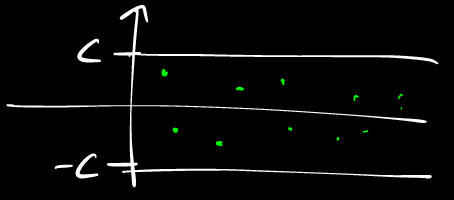
\includegraphics[width=0.9\textwidth]{../../GlobalMedia/sequence-bounded}\\~\\
 \includegraphics[width=0.9\textwidth]{../../GlobalMedia/sequence-cauchy}
 	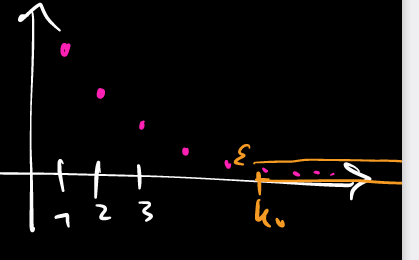
\includegraphics[width=0.9\textwidth]{../../GlobalMedia/sequence-null}
\end{minipage}

\end{defi}
\end{frame}
%
\begin{frame}
% BOUNDED SEQUENCES
\begin{ex}
	\blank 
	Let $a\in\R$. The following sequences are bounded:\\


		i) The constant sequence $\{a\}_{k\in\N}$ (choose $C = a$), \\
		
		ii) The sequence $\{\frac{1}{k}\}_{k\in\N}$ (choose $C = 1$),\\
		
		iii) The \textbf{alternating sequence} $\{a (-1)^k\}_{k\in\N}$ (choose $C=a$). This sequence is not convergent but bounded.

~\\
	An example of an unbounded sequence is given by\\
	
	iv) the sequence $\{k^2\}_{k\in\N}$. \\~\\
	One can show for a sequence $(x^k)_{k\in \N}$ in $\R$:
	$$(x^k)_{k\in \N}~\text{convergent}~\Rightarrow~(x^k)_{k\in \N}~\text{Cauchy}~\Rightarrow~(x^k)_{k\in \N}~\text{bounded}.$$
\end{ex}
\end{frame}

\only<article>{
\begin{frame} 
\begin{theo}[Uniqueness of limits]
	Let $(x^k)_{k\in \N}$ be a sequence in $\R$, then $(x^k)_{k\in \N}$ has at most one limit.
\end{theo}
\only<article>{\begin{proof} \blank
	We proof the statement by contradiction. Therefore, let us assume $(x^k)_{k\in \N}$ converges to $\bar{x}_1$ and $\bar{x}_2$, with $\bar{x}_1\neq \bar{x}_2$. We define $\varepsilon := \frac{1}{2}|\bar{x}_1- \bar{x}_2|>0$. Then by definition of the limit there exist $N_1\in\N$ and $N_2\in\N$ so that
	$$|x^k-\bar{x}_1| <  \ve ~~\text{and}~~|x^k-\bar{x}_2| <  \ve$$
	for all $k \geq \max\{N_1,N_2\}$. Thus, by triangle inequality it follows
	$$2\ve = |\bar{x}_1- \bar{x}_2| =  |\bar{x}_1- (x^k-x^k) -\bar{x}_2| \leq |\bar{x}_1-  x^k|+|x^k- \bar{x}_2| < 2\ve.$$
	Since $2\ve < 2\ve$ is a contraction for $\ve>0$, we have that there cannot exist two distinct limits $\bar{x}_1$ and $\bar{x}_2$ as assumed above.
\end{proof}}
~\\~\\
Important relation between the different types of sequences: \vspace{-0.3cm}
\begin{theo}\label{theo:relation_conv_cauchy_bound}
	Let $(x^k)_{k\in \N}$ be a sequence in $\R$, then 
	$$(x^k)_{k\in \N}~\text{convergent}~\Rightarrow~(x^k)_{k\in \N}~\text{Cauchy}~\Rightarrow~(x^k)_{k\in \N}~\text{bounded}.$$
\end{theo}\vspace{0.4cm}
\only<article>{\begin{proof}\blank
	We only prove the first implication (the second implication requires some more technical steps). For this purpose let $\tilde{\ve} > 0$. Since $(x^k)_{k\in \N}$ is a convergent sequence, there exists a $\bar{x}\in \R$ and a $k_0 \in \N$, so that
	$$|x^m-\bar{x}| <  \tilde{\ve} ~~\text{and}~~|x^n-\bar{x}| <  \tilde{\ve}$$
	for all $m,n \geq k_0$. Thus, by triangle inequality it follows that
	$$|x^m-x^n| = |x^m-(\bar{x}-\bar{x})+x^n| \leq |x^m-\bar{x}| + |x^n-\bar{x}| < 2\tilde{\ve}.$$ Consequently, for $\ve := {\tilde{\ve}}/{2}$ we can choose the same $k_0$ to show the Cauchy property.\\
\end{proof} 
\begin{re}
	Note that by definition, in the ordered field $\R$ all Cauchy sequences also converge. However, this is not true in general! For example, we have seen that the sequence produced by Heron's method does not converge in the ordered field $\Q$, i.e., there is no limit point in $\Q$.
\end{re}}
\textbf{Remark:} In $\R$ all Cauchy sequences also converge (by definition).
\vspace{2.4cm}
\begin{ex}
	\blank
	sequences that are bounded but not cauchy, cauchy but not convergent
\end{ex}
 \end{frame}


%
\begin{frame} 
%
% SUMS AND PRODUCTS OF SEQUENCES
An important tool to compute limits in practice is the following:
\begin{theo}[Sums and products of sequences]
	Let $(x^k)_{k\in \N}$ and $(y^k)_{k\in \N}$ be two sequences in $\R$ with $\lim\limits_{k\to\infty}x^k= \bar{x}$ and $\lim\limits_{k\to\infty}y^k= \bar{y}$. Then
	\begin{itemize}
		\item[i)] $\lim\limits_{k\to\infty} (x^k + y^k) = \lim\limits_{k\to\infty}x^k + \lim\limits_{k\to\infty}x^k = \bar{x}+\bar{y}$;
		\item[ii)] $\lim\limits_{k\to\infty} (x^k\cdot y^k) = \lim\limits_{k\to\infty}x^k \cdot \lim\limits_{k\to\infty}y^k = \bar{x}\cdot\bar{y}$.
	\end{itemize}
	In particular we find for $a \in \R$ that $\lim\limits_{k\to\infty} (x^k + a) = \bar{x} +a$ and $\lim\limits_{k\to\infty} (x^k \cdot a) = \bar{x}\cdot a$ .
\end{theo} 
\only<article>{\begin{proof}
	\blank
	i) We define $z^k := x^k + y^k$ and $\bar{z} := \bar{x} + \bar{y}$. Let $\ve >0$. For ${\tilde{\ve}} := \ve/{2}$ there exists a $k_0 \in \N$, so that
	$$|x^k-\bar{x}| <  \tilde{\ve} ~~\text{and}~~|y^k-\bar{y}| <  \tilde{\ve}$$
	for all $k \geq k_0$. Thus by triangle equality we find
	\begin{align*}
	|z^k - \bar{z}| &= |x^k+y^k - (\bar{x} + \bar{y})| \\
	&= |x^k- \bar{x} +y^k - \bar{y}| \\
	&\leq |x^k- \bar{x}| + |y^k - \bar{y}| \\
	&<  \tilde{\ve}+\tilde{\ve} = \ve.
	\end{align*}

		ii) We define $z^k := x^k \cdot y^k$ and $\bar{z} := \bar{x} \cdot \bar{y}$. First note that by Theorem \ref{theo:relation_conv_cauchy_bound}, we have that the sequence $(x^k)_{k\in \N}$ is bounded, which implies that there exists a bound $C>0$ so that $|x^k| < C$ for all $k\in\N$. By triangle inequality, we find
	\begin{equation} \label{aux1}
	\begin{aligned}
	|z^k - \bar{z}| &= |x^ky^k -  \bar{x}\bar{y}| \\
	&= |x^ky^k - (x^k\bar{y}-x^k\bar{y}) + \bar{x}\bar{y}| \\ 
	&= |x^k(y^k-\bar{y}) +  (x^k-\bar{x})\bar{y}| \\ 
	&\leq  |x^k(y^k-\bar{y})| +  |( \bar{x}-x^k)\bar{y}| \\
	&=  |x^k ||(y^k-\bar{y})| +  |( \bar{x}-x^k)||\bar{y}| \\
	&\leq C |(y^k-\bar{y})| + |( \bar{x}-x^k)||\bar{y}|.
	\end{aligned}
	\end{equation}
	Now let $\ve > 0$. Then for $\tilde{\ve} := \ve / (C+|\bar{y}|) > 0$ there exists a $k_0 \in \N$, so that 
	$$|x^k-\bar{x}| <  \tilde{\ve} ~~\text{and}~~|y^k-\bar{y}| <  \tilde{\ve}$$
	for all $k \geq k_0$. Thus, combining this with \eqref{aux1} 
	gives the desired result
	\begin{align*}
	|z^k - \bar{z}|  < C \tilde{\ve}  + \tilde{\ve} |\bar{y}| = (C+|\bar{y}|)\tilde{\ve}  = \ve.
	\end{align*}
\end{proof}}

\begin{ex}
	\blank Let $a \in \R$.
	\begin{itemize}
		\item[i)] The sequence $\{a + \frac{1}{k}\}_{k\in\N}$
		\item[ii)] The sequence $\{a \cdot\frac{1}{k}\}_{k\in\N}$
		\item[iii)] The sequence $\{ \frac{1}{k^2}\}_{k\in\N}$
	\end{itemize}
\end{ex}
 \end{frame}



 
\begin{frame} 
% SQUEEZE THEOREM
~\\[-15pt]
\begin{theo}[Squeeze theorem]
	Let $(x^k)_{k\in \N}$, $(y^k)_{k\in \N}$ and $\{z^k\}_{k\in \N}$ be sequences in $\R$ with $\lim\limits_{k\to\infty}x^k= \bar{x}$ and $\lim\limits_{k\to\infty}z^k= \bar{x}$. If 
	$$x^k \leq y^k \leq z^k~~~\text{for all}~~~k\in\N,$$
	then also
	$$\lim\limits_{k\to\infty}y^k= \bar{x}.$$
\end{theo}
\begin{proof}\blank
	Let $\ve > 0$, then there exists a $k_0 \in \N$, so that, for all $k \geq k_0$,
	$$|x^k-\bar{x}| <  \tilde{\ve} ~~\text{and}~~|z^k-\bar{y}| <  \tilde{\ve}.$$
	Thus, by definition of the absolute value and the assumptions, we find, for all $k \geq k_0$,
	$$-\ve < x^k-\bar{x} \leq y^k-\bar{x} \leq z^k- \bar{x} < \ve .$$
	This implies $|y^k - \bar{x}|< \ve$ for all $k \geq k_0$.
\end{proof}
 \end{frame}
\begin{frame} 
% BUNCH OF EXAMPLES
\begin{ex}\blank
	Let $f\colon \N \to \N$ with $f(k) \geq 0$ for all $k \in \N$. Then the sequence $\{\frac{1}{k + f(k)}\}_{k\in \N}$ is a null sequence.
\end{ex}
 \end{frame}
}


%%%%%%%%%%%%%%%%%%%%%%%%%%%%%%%%%
% Quadratic equations and inequalities
\mode<article>{
\begin{frame} 
\Subsection{Quadratic equations and inequalities in $\R$}
\only<presentation>{	\tableofcontents[currentsubsection]}
\Subsubsection{Quadratic equations and completion of the square}
We want to solve quadratic equations of the following kind
\begin{align} \label{normalform_quadeq}
x^2 + px +q = 0, 
\end{align}
where $p,q\in \R$ are fixed. Representation \eqref{normalform_quadeq} is sometimes referred to as {\color{defgruen} \textbf{normalized form}} or {\color{defgruen} \textbf{reduced form}}.\\
~\\
Recall the binomial formulas: For $a,b \in \R$ we have
\begin{itemize}
	\item[i)] $(a+b)^2 = a^2 + 2ab + b^2$ 
	\item[ii)] $(a-b)^2 = a^2 - 2ab + b^2$ 
	\item[iii)] $(a+b)(a-b) = a^2 - b^2$ 
\end{itemize}
\vspace{0.3cm}
 \end{frame}


\begin{frame} 
\begin{ex}
	We want to find all $x \in \R$, that satisfy the quadratic equation $$x^2 + 6x + 5 = 0 .$$
\end{ex}

 \end{frame}

\begin{frame} 
In general we find:\\[4pt]
{\color{satzrot} 
	If $\left(\frac{p}{2}\right)^2 \geq q$, then the quadratic equation
	$$  x^2 + px +q = 0 $$
	is solved by
	$$x = -\frac{p}{2} \pm \sqrt{ \left(\frac{p}{2}\right)^2 - q}.$$
}
\begin{proof}
	\blank
\end{proof}
 \end{frame}


%ALTERNATIVE 1
\begin{frame} 
\textbf{Alternative representation (I)}\\[6pt]
Quadratic equations are also often introduced in the following form:
\begin{align} \label{genform_quadeq}
ax^2 + bx + c = 0 
\end{align}
for fixed $a,b,c \in \R$. Representation \eqref{genform_quadeq} is referred to as the {\color{defgruen} \textbf{general form}} of a quadratic equation.\\[5pt]
Assumed $a \neq 0$ we can deduce the reduced form \eqref{normalform_quadeq}:

 \end{frame}

\begin{frame} 
\begin{ex}
	We want to find all $x \in \R$, that satisfy the quadratic equation $$2x^2 + 8x + 6.72 = 0 .$$
\end{ex}
 \end{frame}


%ALTERNATIVE 2
\begin{frame} 
\textbf{Alternative representation (II)}\\[6pt]
Quadratic equations are also introduced as:
\begin{align} \label{vertexform_quadeq}
a(x-h)^2 + k = 0 
\end{align}
for fixed $a,h,k \in \R$. Representation \eqref{vertexform_quadeq} is referred to as {\color{defgruen} \textbf{vertex form}}.\\[5pt]
Again, we can deduce the reduced form:
 \end{frame}





\begin{frame} 
\textbf{Summary}
 \end{frame}

%%%%%%%%%%%%%%%%
\begin{frame} 
\Subsubsection{Inequalities}
Here we make use of the fact that $\R$ is an ordered field. In particular we will exploit the \textbf{monotonicity} property:\\[6pt]
Let $a,b\in \R$ with $a\leq b$. Then
\vspace{-0.24cm}
\begin{itemize}
	\item[1)] $\forall c\in \R\colon ~ a+c\leq b+c$;
	\item[2)] $\forall c\geq 0\colon ~ ac\leq bc$.
\end{itemize}
From 1) and 2) it follows that
$$\forall c< 0\colon ~ ac\geq bc $$
 \end{frame}


\begin{frame} 
\begin{ex}
	We want to find all $x \in \R$, that satisfy the inequality $$x^2 + 6x + 5 \geq 0 .$$
\end{ex}
 \end{frame}



\begin{frame} 
\begin{ex}
	We want to find all $x \in \R$, that satisfy the inequality $$2x \geq 5x-6.$$
\end{ex}
 \end{frame}


\begin{frame} 
\begin{ex}
	We want to find all $x \in \R$, that satisfy the inequality $$\frac{x+4}{4x-12}  \leq 2.$$
\end{ex}
 \end{frame}

}
